\section{Kombination und Selektion}\label{sec:eltern}
\subsection{Kombination}
Da die länge des Genstringst in diesem Beispiel sehr lange ist, bietet es sich an einen Multi-Point-Crossover zu verwenden.
Dabei werden die beiden Eltern an $n$ zufällig gewählten Stellen geterennt und auf zwei neue Genstrings aufgeteilt.
\autoref{img:multiCrossover} zeigt anschaulich wie ein 3-Point-Crossover funktioniert. An je mehr Punkten
der Genstring geteilt und wieder zusammengesetz wird desto einen großeren Unterschied besitzen die Kinder von
den Eltern. Das Crossover an 3 Punkten bietet sich in dieser Anwendung an, da so der Unterschied nicht zu groß aber auch nicht zu klein ist.

\begin{figure}[h]
    \begin{minipage}{\textwidth}
	    \centering
        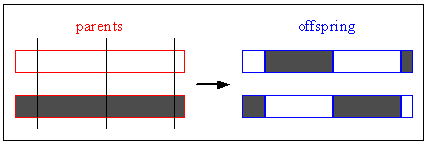
\includegraphics{multiPointCrossover.PNG}
	    \caption{Multi-Point-Crossover {http://www.geatbx.com}}
        \label{img:multiCrossover}
    \end{minipage}
\end{figure}

\subsection{Selektion}
Für die Selektion der Eltern bietet sich die Tournament Selection an.
Diese wählt zufällig mehrere Chromosome aus und selektiert das Chromosom mit der besten Fitness. Das Verfahren der
Tournament Selection ist in \autoref{img:tournament} dargestellt.


\begin{figure}
    \begin{minipage}{\textwidth}
        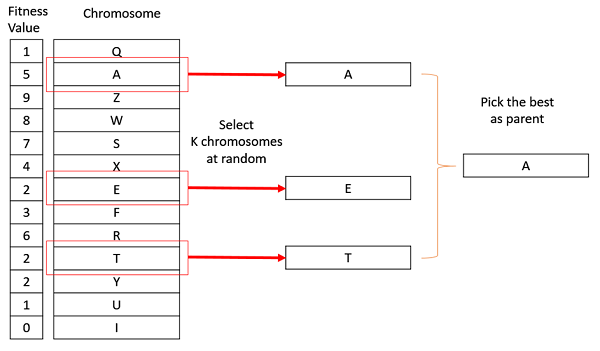
\includegraphics[width=\textwidth]{tournament_selection.jpg}
        \caption{Tournament Selection {https://www.tutorialspoint.com}}
        \label{img:tournament}
    \end{minipage}
\end{figure}

Da eine Population etwa 25 Gene besitzt, sollten für die Tournament Selection nicht mehr als 4 Chromosome zufällig gewählt werden.
Würden zu viele Chromosome gewählt werden, könnten auch einfach die besten zwei Gene der Population ausgewählt werden.
Dies würde zu wenig veränderung der Gene führen und könnte dafür sorgen, dass nicht das globale sondern
lediglich ein lokales Optimum gefunden wird.

Ein Ansatz der genauer untersucht werden sollte ist es, an einem Zeitpunkt gegen Ende der
Evolution die Tournament Selection mit einer Zufall-Selektion auszutauschen.
Dies hat den Grund, dass zu diesem Zeitpunkt angenommen werden kann, dass alle
Gene eine ähnliche Fitness besitzen.